\section{Introduction}
\emph{Credit Payment Services}, such as offline credit card services in commercial banks and online credit payments in internet financial institutions, are widely used in many aspects of daily life and bring convenience to both users and merchants. However, ever-increasing frauds have seriously influenced the security of credit payment services.  
\emph{Cash-out} fraud is to pursue cash gains with illegal or insincere means, e.g., through buying pre-paid cards or other goods then reselling them. 
With the rapid development of e-commerce, it has become one of the major frauds on various kinds of credit payment services. 
Cash-out fraud behavior is illegal and may cause financial venture, since the probability of loan default is much higher for cash-out users in most cases. 
Therefore, \emph{cash-out user detection} becomes one of the most important components of the fraud detection system in financial institutions.

The goal of cash-out user detection is to predict whether a user will do cash-out transactions or not in the future.
Thus this problem can be formulated as a classification problem.
Conventional solutions first perform subtle feature engineering for each user, and then a classifier, such as tree-based model or neural network, is trained based on these features.
The key point of these methods is to extract statistical features of users from different aspects, such as user profile, credit history, transaction summarizing, and recent behaviors in other relative businesses.
Conventional methods make prediction mainly based on the statistical features of a certain user, but seldom fully exploit the interaction relations between users, which may be beneficial to the cash-out user detection problem.

\begin{figure}[t]
\centering
\subfigure[Scenario of credit payment service]{
  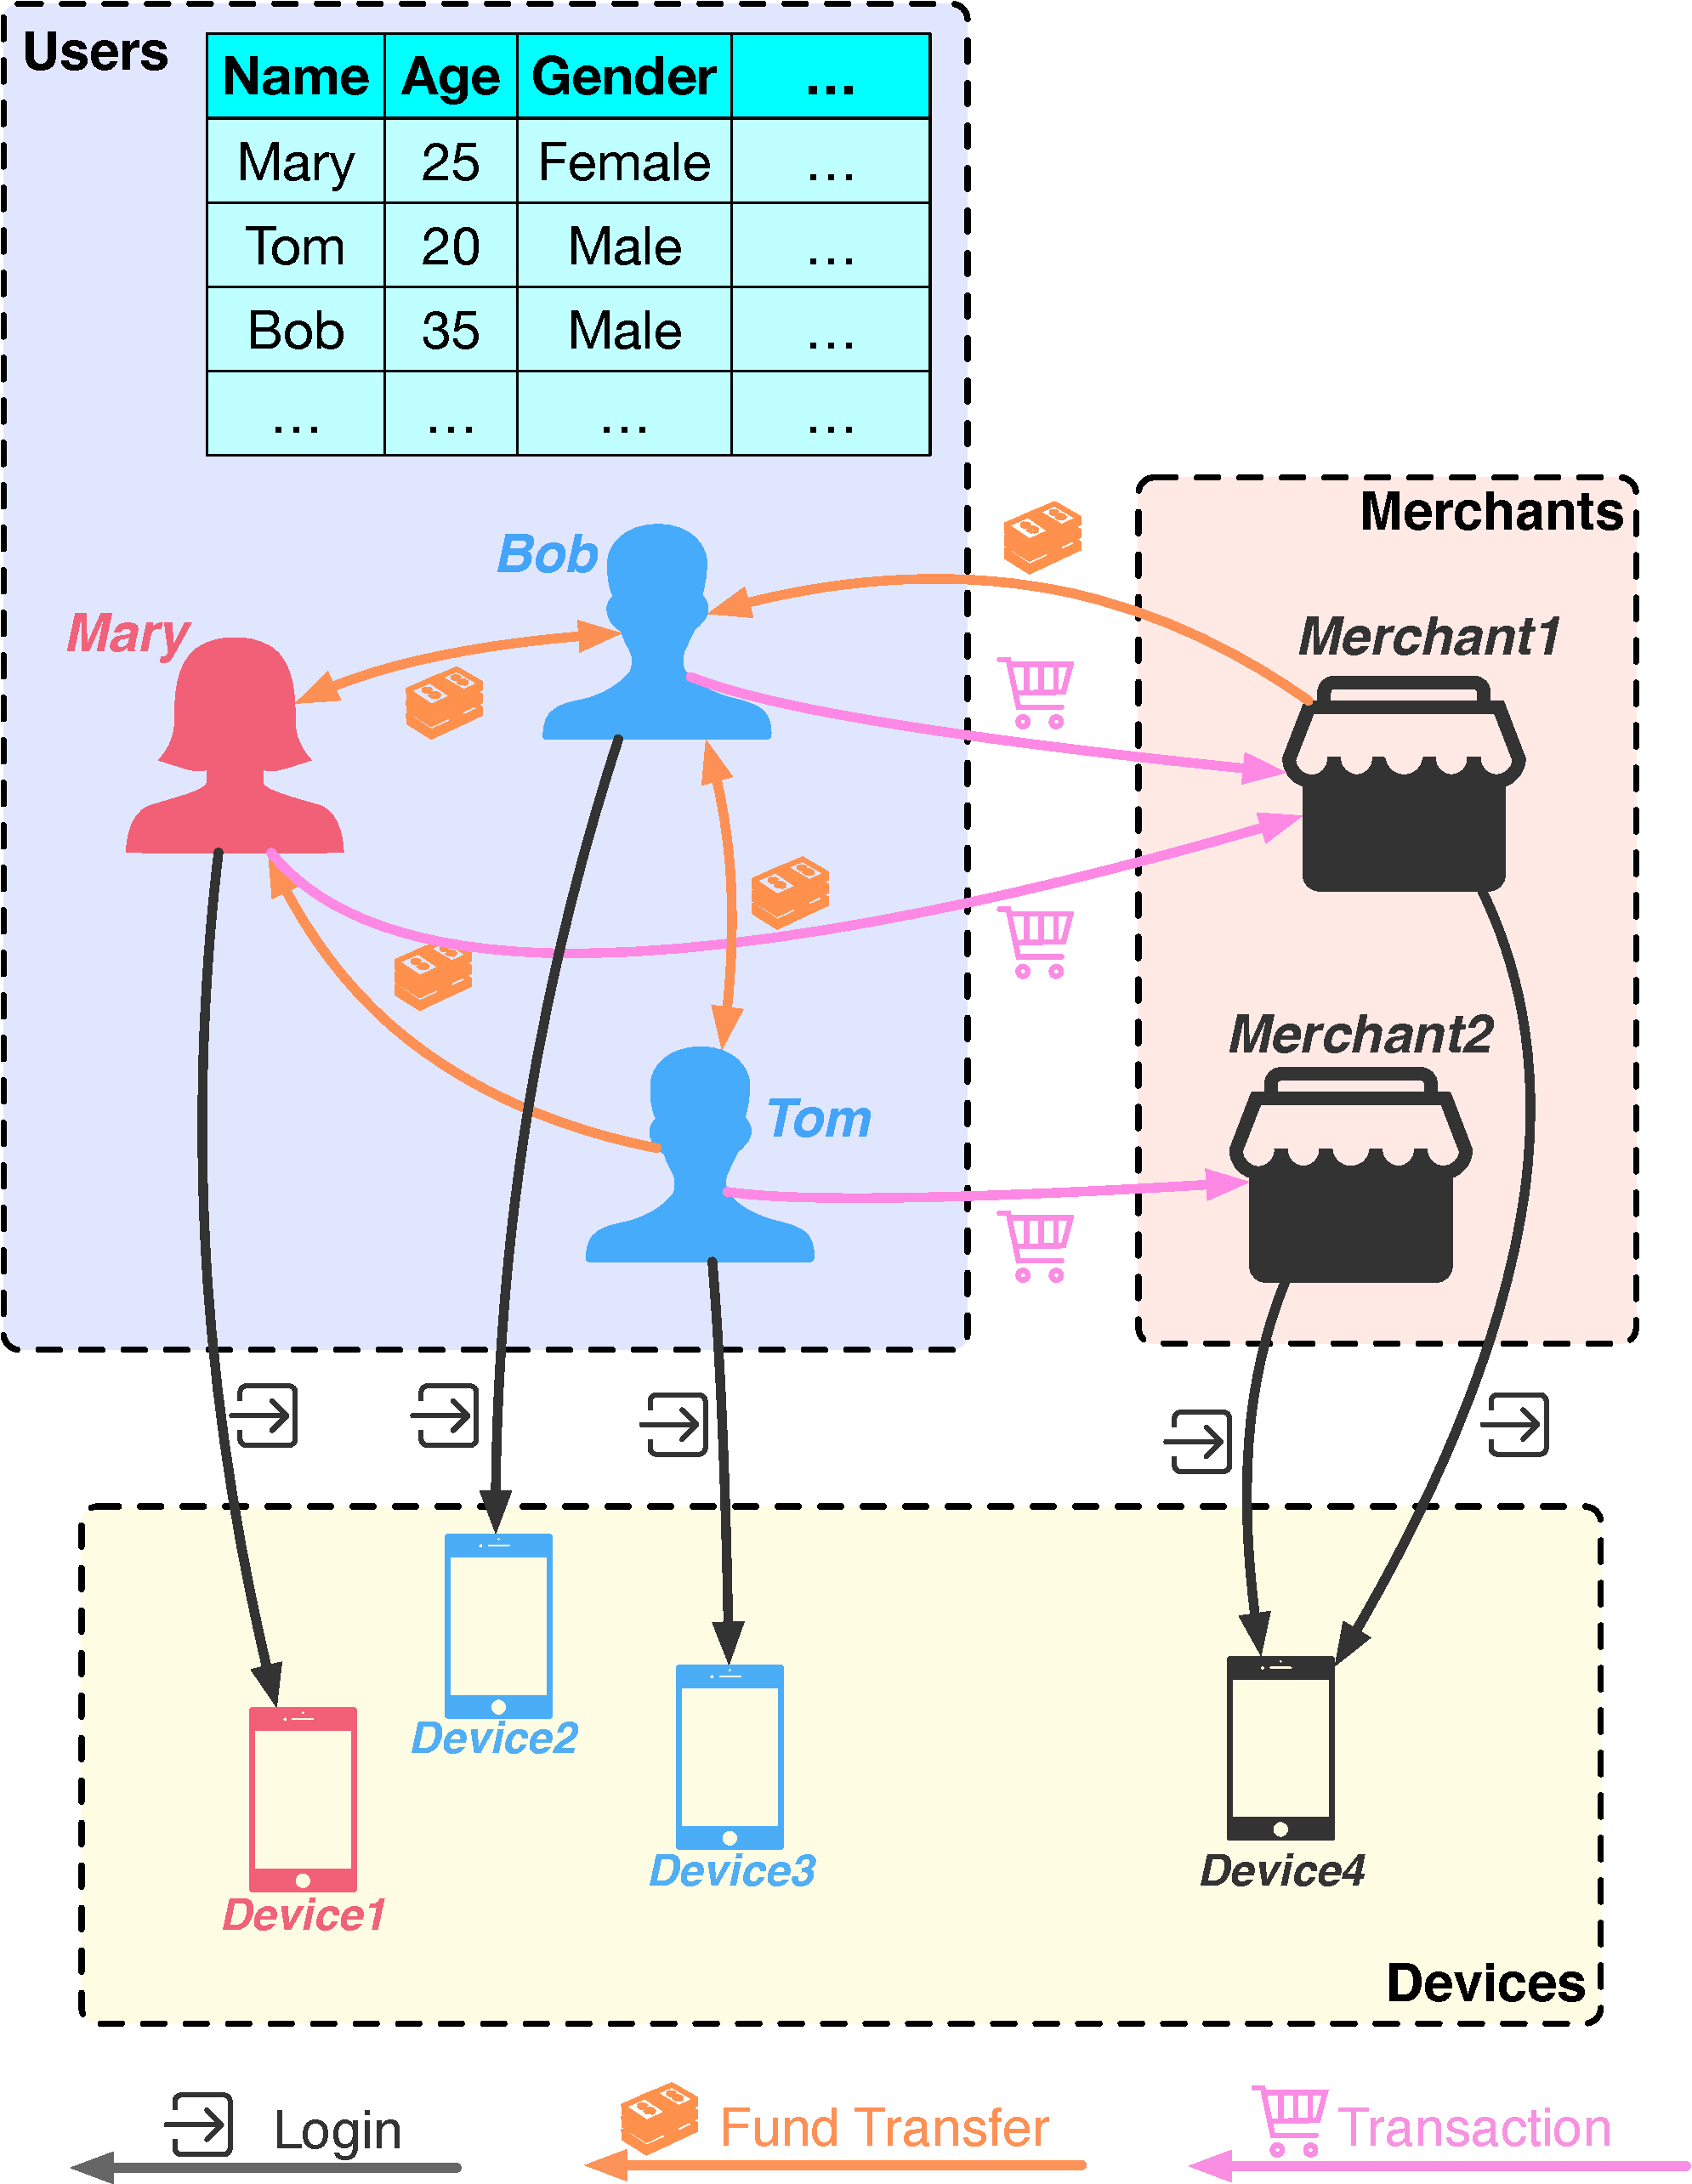
\includegraphics[width=4.5cm]{image/HIN_demo_2.pdf}\label{fig-hin}}
\subfigure[Network schema and meta-path examples]{
  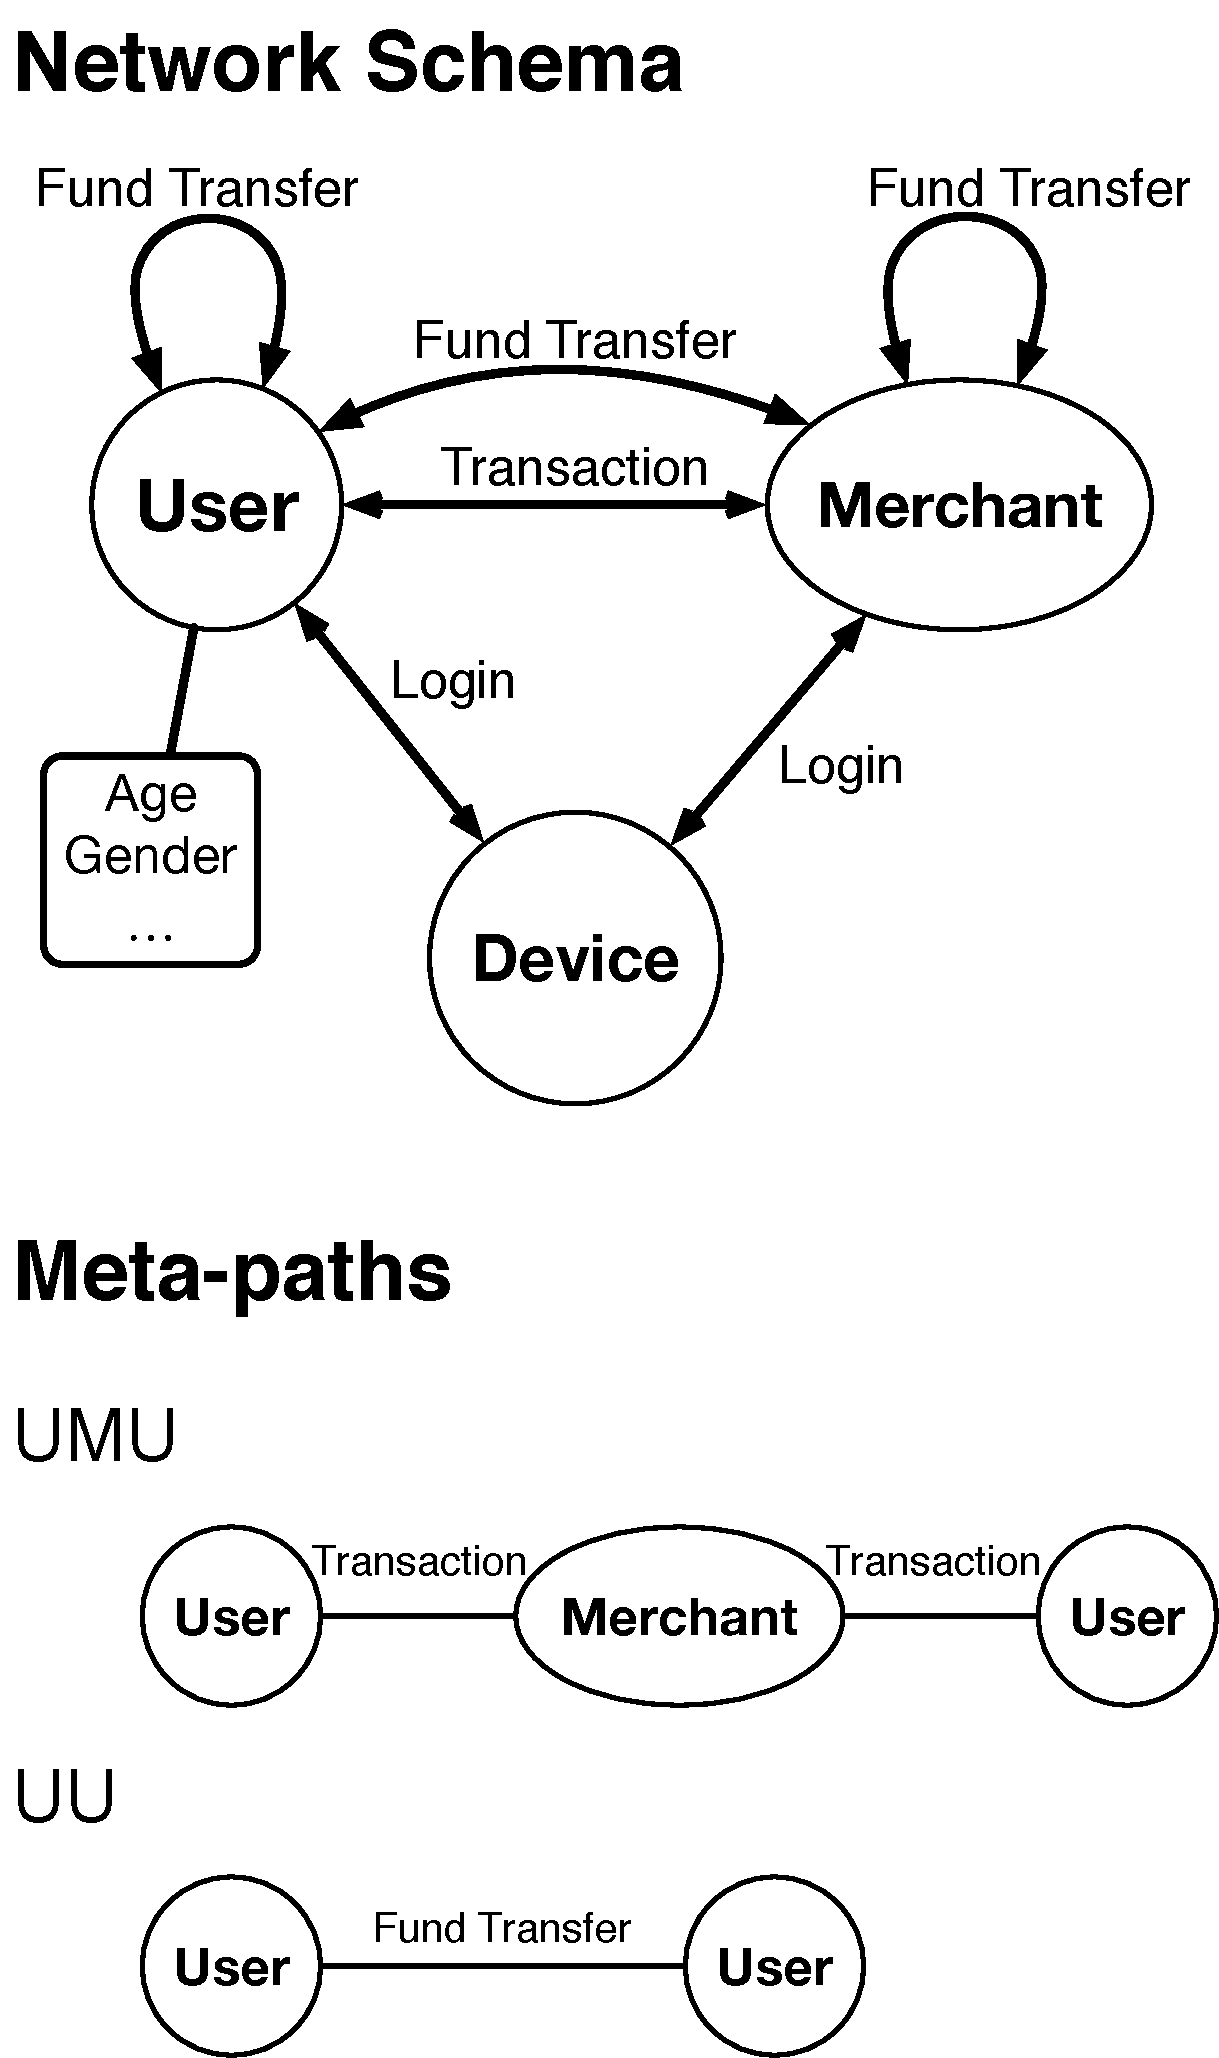
\includegraphics[width=3.5cm]{image/HIN_schema.pdf}\label{fig-hin_schema}}
\caption{The AHIN of the scenario of credit payment service.}
\label{fig:network_analysis}
\end{figure}


In fact, there are rich interaction relations in the scenario of credit payment service, which are really important to the cash-out user detection problem.  
Fig. \ref{fig-hin} demonstrates a general scenario of credit payment service, where there are three types of objects: users, merchants, and devices (the way to access services, e.g., websites, desktops, mobile apps, wifi devices, etc.). 
Besides the attribute information, these objects also have rich interaction information \eg the fund transfer relation among users, the login relation between users and devices, and the transaction relation between users and merchants. 
The cash-out users not only have abnormal features, but also behavior abnormally in interaction relations. 
For example, the cash-out users may simultaneously have many transaction and fund transfer interactions with particular merchants, which is hard to be exploited by traditional feature extraction. 

In order to exploit the interaction relations and feature information, we propose to model the scenario of credit payment service with an \emph{\textbf{A}ttributed \textbf{H}eterogeneous \textbf{I}nformation \textbf{N}etwork} (AHIN). 
The recently emerging \emph{\textbf{H}eterogeneous \textbf{I}nformation \textbf{N}etwork} (HIN)~\citep{shi2017survey}, consisting of multiple types of nodes and links, has been proposed as a powerful information modeling method for characterizing data heterogeneity~\citep{sun2011pathsim,zhao2017meta}. 
Furthermore, in order to incorporate the attribute information of objects, we extend traditional HIN to AHIN, where objects in HIN may contain attributes (or termed as features). 
Fig.~\ref{fig-hin_schema} shows the network schema of the AHIN in the scenario of credit payment service, which clearly illustrates the objects and their interactions. 
Several efforts have been made for mining HIN and shown promising performance in various kinds of applications~\citep{dong2017metapath2vec,sun2012mining,shi2018heterogeneous}.
However, they are usually designed for specific task and only exploit structure information, so they cannot be directly applied for the AHIN and the cash-out user detection problem. 

In this paper, we first study the cash-out detection problem under the AHIN framework, and propose a novel \textbf{H}ierarchical \textbf{A}ttention mechanism based \textbf{C}ash-out \textbf{U}ser \textbf{D}etection model, called HACUD. The basic idea of HACUD is to significantly enhance the feature representation of objects through fully exploiting interaction relations, i.e., with the help of meta-path based neighbors in AHIN. Inspired by~\citep{Kipf2016Semi,zhang2018anrl} and our observations on real data, we assume that the feature representation of objects, besides intrinsic features, are also constituted by the features of their neighbors. We propose the concept of meta-path based neighbors to exploit rich structure information in AHIN. That is, we can find neighbors of a node through the assigned meta-path (a relation sequence connecting two nodes). It has several advantages: (1) It can capture different aspects of structure information through different meta-paths~\citep{han2018aspect}; (2) It greatly reduces the dimension of representation space, compared to traditional network representation learning methods; (3) It is potential to predict new-coming nodes dynamically. Furthermore, we assume that object attributes and meta-paths have different importances, and elaborately design a hierarchical attention mechanism to learn user preferences towards attributes and meta-paths. Specifically,  the first layer of our attention mechanism models the user's attention in the feature space (\ie attributes), while the second layer captures the different contributions of different meta-paths for the prediction task. Finally, a cash-out probability is predicted based on aggregated feature representation with a multi-layer perceptron. 

In summary, our work has the following contributions. 

\textbullet \  We are the first to study the cash-out users detection problem, which is a very important and widely existing problem in financial fraud field. 

\textbullet \  We propose to model the cash-out user detection problem as a classification problem in AHIN which is constituted by different types of objects and their rich interactions in the scenario
of credit payment service.

\textbullet \  We propose a novel model HACUD to solve the problem, which employs meta-path based neighbors to fully exploit structure information and a hierarchical attention mechanism to automatically learn the importance of attributes and meta-paths. 

\textbullet \  Extensive experiments on two real datasets illustrate the best performance of the proposed HACUD compared to the state of arts, as well as the benefits of hierarchical attention mechanism.
%in cash-out user detection problem shows that our proposal outperforms several state-of-the-art methods.
      
